%%%%%%%%%%%%%%%%%%%%%%%%%%%%%%%%%%%%%%%%%%%%%%%%%%%%%%%%%%%%%%%%%%%%%%%%%%%%%%%%
\section{A first Workflow}
{   
	\usebackgroundtemplate{
		\vbox to \paperheight{\vfil\hbox to \paperwidth{\hfil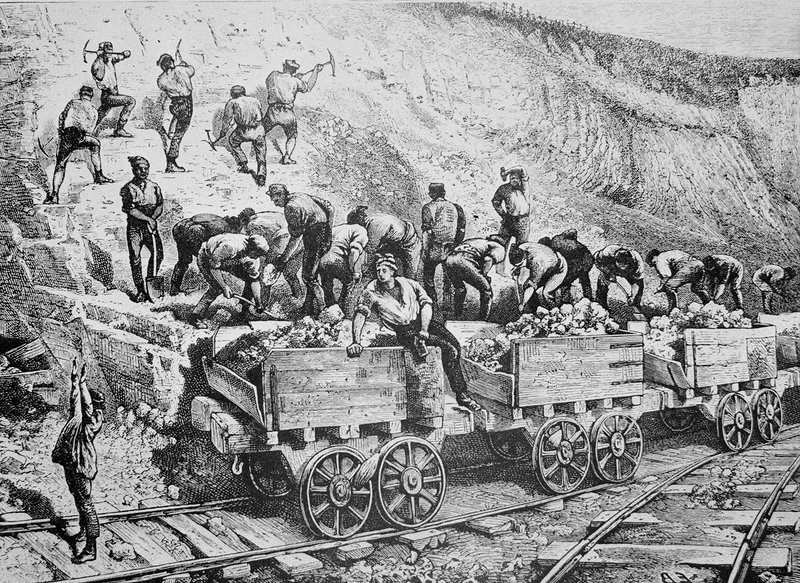
\includegraphics[height=\paperheight]{logos/Railway_construction,_19th_century.jpg}\hfil}\vfil}
	}
	\frame{
		\frametitle{Finally: Work!}
		\begin{mdframed}[tikzsetting={draw=white,fill=white,fill opacity=0.8,
				line width=0pt},backgroundcolor=none,leftmargin=0,
			rightmargin=150,innertopmargin=4pt,roundcorner=10pt]
			\tableofcontents[currentsection,sections={1-4},hideothersubsections]
		\end{mdframed}
	}
}

%%%%%%%%%%%%%%%%%%%%%%%%%%%%%%%%%%%%%%%%%%%%%%%%%%%%%%%%%%%%%%%%%%%%%%%%%%%%%%%%
\begin{frame}
  \frametitle{What is this about?}
   \begin{question}[Questions]
   	 How do I write a simple workflow?
   \end{question}
   \begin{docs}[Objectives]
   	 \begin{enumerate}
                      \item Understand the components of a Snakefile: rules, inputs, outputs, and actions.
                      \item Write a simple Snakefile.
                      \item Run Snakemake from the shell.
                      \item Learning what a "target" stands for and to use it.
     \end{enumerate}
   \end{docs}
\end{frame}

%%%%%%%%%%%%%%%%%%%%%%%%%%%%%%%%%%%%%%%%%%%%%%%%%%%%%%%%%%%%%%%%%%%%%%%%%%%%%%%
\begin{frame}[fragile]
  \frametitle{Before we begin \ldots}
  \begin{exampleblock}{Working with closure Files}
    To ease the excercises and save typing time, all exercises are supplied as cloze texts.\linebreak
    \Snakemake{} relies on a file called \altverb{Snakefile} to be present. You can either rename your cloze texts like
    \begin{lstlisting}[language=Bash, style=Shell]
$ cp <number>_Snakefile Snakefile
    \end{lstlisting}
    or specify the workflow file on the command line with an additional flag:
    \begin{lstlisting}[language=Bash, style=Shell]
$ snakemake <other arguments> \
> --snakefile <number>_Snakefile
    \end{lstlisting}
    Also note: \altverb{\\} may denote a linebreak in \texttt{Bash} and \altverb{>} its continuation. Omit these and you have a one-liner. It merely serves to fit text on screen, here.
  \end{exampleblock}
\end{frame}

%%%%%%%%%%%%%%%%%%%%%%%%%%%%%%%%%%%%%%%%%%%%%%%%%%%%%%%%%%%%%%%%%%%%%%%%%%%%%%%%
\begin{frame}[fragile]
	\frametitle{Specifiying Snakefiles (Details)}
	% impossible to use \Snakemake command in environment header
	\begin{docs}[Snakemake's default \altverb{Snakefile}]
		The workflow definition in form of a snakefile. Usually, you should not need to specify this. By default, \Snakemake{} will search for "\altverb{Snakefile}", "\altverb{snakefile}","\altverb{workflow/Snakefile}", \\"\altverb{workflow/snakefile}" beneath the current working directory, in this order.\newline
		When using a different layout, you can use
		\begin{lstlisting}[language=Bash, style=Shell]
$ snakemake <other arguments> \
> --snakefile <path to snakefile>
	    \end{lstlisting}
	\end{docs}
    \pause
    \begin{hint}
      On clusters we recommend working from \altverb{HOME} and configuring workflows such that they point to data on project file systems. How and the reasons why will be covered.
    \end{hint}
\end{frame}


%%%%%%%%%%%%%%%%%%%%%%%%%%%%%%%%%%%%%%%%%%%%%%%%%%%%%%%%%%%%%%%%%%%%%%%%%%%%%%%%
\subsection{A first Step or ``Rule''}

%%%%%%%%%%%%%%%%%%%%%%%%%%%%%%%%%%%%%%%%%%%%%%%%%%%%%%%%%%%%%%%%%%%%%%%%%%%%%%%%
\begin{frame}[fragile]
  \frametitle{Layout of a Workflow Development Directory} 
  The idea is to have a neat overview:
  \begin{columns}
    \begin{column}{0.5\textwidth}
      
  \begin{minipage}[t]{0.5\textwidth}
    \setstretch{0.1}
            {\tiny \DTsetlength{0.2em}{1em}{0.2em}{0.4pt}{.6pt}
\dirtree{%
.1 {\textit{workflow\ folder}}.
.2 {scripts}.
.3 {some\_scriptfile.py}.
.3 {some\_scriptfile.sh}.
.3 {some\_scriptfile.R}.
.2 {Snakefile}.
.2 {and more \ldots}.
}}
    \end{minipage}
    \end{column}
    \begin{column}{0.5\textwidth}
      \begin{hint}
      	Our long term goal:\newline Have a orderly overview and seperation of data and code. We will start with one \altverb{Snakefile}.
      \end{hint}
    \end{column}
  \end{columns}
\end{frame}

%%%%%%%%%%%%%%%%%%%%%%%%%%%%%%%%%%%%%%%%%%%%%%%%%%%%%%%%%%%%%%%%%%%%%%%%%%%%%%%%
\begin{frame}[fragile]
  \frametitle{Our first Snakefile!}
  \begin{onlyenv}<1| handout:0>
    Our first ``\altverb{rule}''; we want to map reads onto a reference genome. 
    \begin{lstlisting}[language=Python,style=Python]
rule bwa_map:
    input:
        "data/genome.fa",
        "data/samples/A.fastq"
    output:
        "mapped_reads/A.bam"
    shell:
        "bwa mem data/genome.fa"
        " data/samples/A.fastq"
        " | samtools view -Sb - >"
        " mapped_reads/A.bam"
    \end{lstlisting}
    \begin{docs}
    	This code is build file, which for \Snakemake{} is called a \altverb{Snakefile} -- a file executed by \Snakemake{}.
    \end{docs}
    \end{onlyenv}
  \begin{onlyenv}<2| handout:0>
   We are going to ``map'' our reads onto the genome.
   \begin{lstlisting}[language=Python,style=Python]
rule @bwa_map@:
    input:
        "data/genome.fa",
        "data/samples/A.fastq"
    output:
        "mapped_reads/A.bam"
    shell:
        "bwa mem data/genome.fa"
        " data/samples/A.fastq"
        " | samtools view -Sb - >"
        " mapped_reads/A.bam"
    \end{lstlisting}
    For this we are using \lhref{https://github.com/lh3/bwa}{\altverb{bwa}}, specifically \altverb{bwa mem}. We call our rule accordingly \altverb{bwa_map}.
  \end{onlyenv}
  \begin{onlyenv}<3| handout:0>
   \altverb{input}, \altverb{output} and \altverb{shell} are called ``directives'':
   \begin{lstlisting}[language=Python,style=Python]
rule bwa_map:
    @input@:
        "data/genome.fa",
        "data/samples/A.fastq"
    @output@:
        "mapped_reads/A.bam"
    @shell@:
        "bwa mem data/genome.fa"
        " data/samples/A.fastq"
        " | samtools view -Sb - >"
        " mapped_reads/A.bam"
    \end{lstlisting}
    The \altverb{input} and \altverb{output} directives are followed by lists of files that are expected to be used or created by the rule. In the simplest case, these are just explicit Python strings.
  \end{onlyenv}
  \begin{onlyenv}<4| handout:0>
   The \altverb{shell} directive contains one ore more lines ($+$ line breaks) and sets the command executed on the Shell:
  \begin{lstlisting}[language=Python,style=Python]
rule bwa_map:
    input:
        "data/genome.fa",
        "data/samples/A.fastq"
    output:
        "mapped_reads/A.bam"
    shell:
        @"bwa mem data/genome.fa"
        " data/samples/A.fastq"
        " | samtools view -Sb - >"
        " mapped_reads/A.bam"@
    \end{lstlisting}
    \bcattention Python will concatenate those Strings! Be sure to include spaces to make up a valid command in Bash.
  \end{onlyenv}
  \begin{onlyenv}<5| handout:1>
   Be sure to have copied everything to your \altverb{Snakefile} and save it.
   \begin{lstlisting}[language=Python,style=Python]
rule bwa_map:
    input:
        "data/genome.fa",
        "data/samples/A.fastq"
    output:
        "mapped_reads/A.bam"
    shell:
        "bwa mem data/genome.fa"
        " data/samples/A.fastq"
        " | samtools view -Sb - >"
        " mapped_reads/A.bam"
    \end{lstlisting}
    You will find working content in the file \altverb{01_Snakefile} in your tutorial folder, too.
  \end{onlyenv}
\end{frame}

%%%%%%%%%%%%%%%%%%%%%%%%%%%%%%%%%%%%%%%%%%%%%%%%%%%%%%%%%%%%%%%%%%%%%%%%%%%%%%%%
\begin{frame}
  \frametitle{Snakefiles are Python Files}
  \begin{block}{Some Background}
     \begin{enumerate}[<+->]
       \item Like Python, you can use either tabs or spaces for indentation — don’t mix! Consensus is to only use \emph{spaces}.
       \item Together, the target, dependencies, and actions form a rule. A rule is a recipe for how to make things.
  \end{enumerate}
  \end{block}
\end{frame}

%%%%%%%%%%%%%%%%%%%%%%%%%%%%%%%%%%%%%%%%%%%%%%%%%%%%%%%%%%%%%%%%%%%%%%%%%%%%%%%%
\begin{frame}[fragile]
  \frametitle{Testing our Snakefile}
  When a workflow is executed, \Snakemake{} tries to generate given target files. Target files can be specified via the command line. By executing
  \begin{lstlisting}[language=Bash, style=Shell]
$ snakemake -np mapped_reads/A.bam
  \end{lstlisting}
  in the working directory containing the \altverb{Snakefile}, we tell \\\Snakemake{} to generate the target file \altverb{mapped_reads/A.bam}.\newline
  We are using 
  \begin{itemize}[<+->]
   \item \altverb{-n/--dry-run} to show the \emph{planned} execution and
   \item \altverb{-p} to print the intended shell command.
  \end{itemize} 
\end{frame}

%%%%%%%%%%%%%%%%%%%%%%%%%%%%%%%%%%%%%%%%%%%%%%%%%%%%%%%%%%%%%%%%%%%%%%%%%%%%%%%%
\begin{frame}[fragile]
  \frametitle{Finally - Running \Snakemake{}!}
  Now, we can run \Snakemake{}:
  \begin{lstlisting}[language=Bash, style=Shell]
$ snakemake --cores=1 mapped_reads/A.bam
  \end{lstlisting}
  \begin{hint}[Note:]
  	The \altverb{--cores=1} is necessary, because we are executing ``locally'' and \Snakemake{} would like to know how much of the resources we may use (you can try without, though, to see what happens).
  \end{hint}
  You should see the expected output (\altverb[Bash]{ls}) and lines which reads:
  \begin{lstlisting}[style=Plain, basicstyle=\footnotesize]
1 of 1 steps (100%) done
Complete log: .snakemake/log/<date>T<timestring>.snakemake.log
  \end{lstlisting}
\end{frame}

%%%%%%%%%%%%%%%%%%%%%%%%%%%%%%%%%%%%%%%%%%%%%%%%%%%%%%%%%%%%%%%%%%%%%%%%%%%%%%%%
\begin{frame}[fragile]
  \frametitle{Re-Running Workflows}
  Try to run \Snakemake{} again:
  \begin{lstlisting}[language=Bash, style=Shell]
$ snakemake --cores=1 mapped_reads/A.bam
  \end{lstlisting}
  \pause
  Oops:
  \begin{lstlisting}[style=Plain, basicstyle=\footnotesize]
Nothing to be done (all requested files are present and up to date).
  \end{lstlisting}
  \begin{question}
  	What happens? Why?
  \end{question}
\end{frame}

%%%%%%%%%%%%%%%%%%%%%%%%%%%%%%%%%%%%%%%%%%%%%%%%%%%%%%%%%%%%%%%%%%%%%%%%%%%%%%%%
\begin{frame}
  \frametitle{When do Rules get executed? - The Solution}
  When it is asked to build a target, \Snakemake{} checks the “last modification time” of both the \emph{target} and its \emph{dependencies}.
  If either
  \begin{itemize}
   \item any dependency has been updated
   \item or a job failed to produce a target (completely)
  \end{itemize}
  upon re-run \Snakemake{} will only rebuild the files that, either directly or indirectly, depend on the file that changed. This is called an \emph{incremental build}.
  \pause
  \begin{docs}
  	By explicitly recording the inputs to and outputs from steps in our analysis and the dependencies between files, \altverb{Snakefile}s act as a type of documentation, reducing the number of things we have to remember.
  \end{docs}
\end{frame}

%%%%%%%%%%%%%%%%%%%%%%%%%%%%%%%%%%%%%%%%%%%%%%%%%%%%%%%%%%%%%%%%%%%%%%%%%%%%%%%%
\begin{frame}[fragile]
  \frametitle{Too much Typing!1!11!}
  A closer look on our first rule reveals:
  \begin{lstlisting}[language=Python,style=Python]
rule bwa_map:
    input:
        "data/genome.fa",
        "data/samples/A.fastq"
    output:
        "mapped_reads/A.bam"
    shell:
        "bwa mem data/genome.fa"
        " data/samples/A.fastq"
        " | samtools view -Sb - >"
        " mapped_reads/A.bam"
    \end{lstlisting}
    \bcattention Way too much redundancy!
\end{frame}

%%%%%%%%%%%%%%%%%%%%%%%%%%%%%%%%%%%%%%%%%%%%%%%%%%%%%%%%%%%%%%%%%%%%%%%%%%%%%%%%
\begin{frame}[fragile]
	\frametitle{\HandsOn{Introducing Wildcards}}
	\altverb{\{input\}} and \altverb{\{output\}} are so-called "wildcards": We can use them 
	to reference our in- and output in the \altverb{shell} directive, e.\,g.:
	\begin{lstlisting}[language=Python,style=Python]
rule foo:
   input: replicate_1.txt,
          replicate_2.txt
   output: result.txt
   # The following command will concatenate
   # the input files.
   shell: "cat {input} > {output}"
    \end{lstlisting}
    \begin{docs}
      If the in-/output has multiple lines, like in this example, \Snakemake{} will concatenate them, separated by a whitespace. In other words \altverb{\{input\}} will contain \altverb{replicate_1.txt replicate_2.txt}.
    \end{docs}
\end{frame}

%%%%%%%%%%%%%%%%%%%%%%%%%%%%%%%%%%%%%%%%%%%%%%%%%%%%%%%%%%%%%%%%%%%%%%%%%%%%%%%%
\begin{frame}[fragile]
	\frametitle{\HandsOn{Introducing Wildcards}}
	\begin{task}
	   Your task is simple to introduce the \altverb{\{input\}} and \altverb{\{output\}}  wildcards in our current \altverb{bwa_map} rule. Replace the input and output within the \altverb{shell} directive using these wildcards.
	\end{task}
    \begin{hint}
       Remember, \Snakemake{} will concatenate multiline in- or output. Refer to  \altverb{02_Snakefile} in your tutorial folder for the task setting.
    \end{hint}
\end{frame}

%%%%%%%%%%%%%%%%%%%%%%%%%%%%%%%%%%%%%%%%%%%%%%%%%%%%%%%%%%%%%%%%%%%%%%%%%%%%%%%%
\begin{frame}[fragile]
  \frametitle{Introducing Wildcards - The "Solution"}
  Now, \altverb{\{input\}} and \altverb{\{output\}} reference the in- and output:
  \begin{lstlisting}[language=Python,style=Python]
rule bwa_map:
    input:
        "data/genome.fa",
        "data/samples/A.fastq"
    output:
        "mapped_reads/A.bam"
    shell:
        "bwa mem {input}"
        " | samtools view -Sb - >"
        " {output}"
    \end{lstlisting}
    Since the rule has multiple input files, \Snakemake{} will concatenate them, separated by a whitespace. In other words, \Snakemake{} will replace \altverb{\{input\}} with \altverb{data/genome.fa data/samples/A.fastq} before executing the command.\newline
    A working example can be found in \altverb{02_Snakefile} in the solution folder.
\end{frame}

%%%%%%%%%%%%%%%%%%%%%%%%%%%%%%%%%%%%%%%%%%%%%%%%%%%%%%%%%%%%%%%%%%%%%%%%%%%%%%%%
\begin{frame}[fragile]
  \frametitle{\HandsOn{Further Workflow Decoration}}
  (Usually), experiments consists of more than one input, e.\,g. several replicas might be present.\newline
  \begin{task}{Introducing the \altverb{sample} Wildcard}
    \Snakemake{} allows generalizing rules by using named wildcards, too. Simply replace the \altverb{A} in the second input file and in the output file with the wildcard \altverb{\{sample\}}.\newline
    You may refer to the \altverb{03_Snakefile} template in your tutorial folder.
  \end{task}
\end{frame}

%%%%%%%%%%%%%%%%%%%%%%%%%%%%%%%%%%%%%%%%%%%%%%%%%%%%%%%%%%%%%%%%%%%%%%%%%%%%%%%%
\begin{frame}[fragile]
  \frametitle{Further Workflow Decoration -- Solution} 
  \footnotesize 
  \Snakemake{} allows generalizing rules by using named wildcards. Simply replace the \altverb{A} in the second input file and in the output file with the wildcard \altverb{\{sample\}}, to yield:
  \begin{lstlisting}[language=Python,style=Python,basicstyle=\footnotesize]
rule bwa_map:
    input:
        "data/genome.fa",
        "data/samples/{sample}.fastq"
    output:
        "mapped_reads/{sample}.bam"
    shell:
        "bwa mem {input} | samtools view -Sb - > {output}"
  \end{lstlisting}
  When \Snakemake{} determines that this rule can be applied to generate a target file by replacing the wildcard \altverb{\{sample\}} in the output file with an appropriate value, it will propagate that value to all occurrences of \altverb{\{sample\}} in the input files and thereby determine the necessary input for the resulting job. 
\end{frame}

%%%%%%%%%%%%%%%%%%%%%%%%%%%%%%%%%%%%%%%%%%%%%%%%%%%%%%%%%%%%%%%%%%%%%%%%%%%%%%%%
\begin{frame}[fragile]
  \frametitle{Execution}
  When executing
  \begin{lstlisting}[language=Bash, style=Shell]
$ snakemake -np mapped_reads/B.bam
  \end{lstlisting}
  \Snakemake{} will determine that the rule \altverb{bwa_map} can be applied to generate the target file by replacing the wildcard \altverb{\{sample\}} with the value \altverb{B}.\newline
  To analyse samples \altverb{A} and \altverb{B}, we can specify two targets
    \begin{lstlisting}[language=Bash, style=Shell]
$ snakemake -np mapped_reads/A.bam mapped_reads/B.bam
  \end{lstlisting}
  or use \lhref{https://tldp.org/LDP/Bash-Beginners-Guide/html/sect_03_04.html}{Bash's brace expansion}
  \begin{lstlisting}[language=Bash, style=Shell]
$ snakemake -np mapped_reads/{A,B}.bam
  \end{lstlisting}
  \pause
  \begin{hint}{Rest Assured!}
  	We will not need to do all this, when we are finished.
  \end{hint}	
\end{frame}

%%%%%%%%%%%%%%%%%%%%%%%%%%%%%%%%%%%%%%%%%%%%%%%%%%%%%%%%%%%%%%%%%%%%%%%%%%%%%%%%
\begin{frame}
	\frametitle{One Caveat!}
	\begin{alertblock}{Multiple Wildcards}
		You can have multiple wildcards in your file paths, however, to avoid conflicts with other jobs of the same rule, \emph{all output files} of a rule \emph{have to contain exactly the same wildcards}.
	\end{alertblock}
\end{frame}

%%%%%%%%%%%%%%%%%%%%%%%%%%%%%%%%%%%%%%%%%%%%%%%%%%%%%%%%%%%%%%%%%%%%%%%%%%%%%%%%
\begin{frame}[fragile]
  \frametitle{\HandsOn{Sorting Alignments}}
  For later steps, we need the read alignments in the BAM files to be sorted. This can be achieved with the \lhref{https://www.htslib.org/}{\texttt{samtools}} \altverb{sort} command. We add the following rule beneath the \altverb{bwa_map} rule:
  \begin{lstlisting}[language=Python,style=Python]
rule samtools_sort:
    input:
        ...
    output:
        ...
    shell:
        "samtools sort -T sorted_reads/{wildcards.sample} "
        "-O bam {input} > {output}"
  \end{lstlisting}
  \begin{task}
  	Please refer to your template \newline \altverb{04_Snakefile} in the tutorial folder and fill in \altverb{input} and \altverb{output}.
  \end{task}
\end{frame}

%%%%%%%%%%%%%%%%%%%%%%%%%%%%%%%%%%%%%%%%%%%%%%%%%%%%%%%%%%%%%%%%%%%%%%%%%%%%%%%%
\begin{frame}[fragile]
  \frametitle{Sorting Alignments / Using Wildcards Solution}
  \begin{lstlisting}[language=Python,style=Python]
rule samtools_sort:
    input:
        "mapped_reads/{sample}.bam"
    output:
        "sorted_reads/{sample}.bam"
    shell:
        "samtools sort -T sorted_reads/{wildcards.sample} "
        "-O bam {input} > {output}"
  \end{lstlisting}
  You will find this solution in \pathtosolutions{04_Snakefile}
\end{frame}

%%%%%%%%%%%%%%%%%%%%%%%%%%%%%%%%%%%%%%%%%%%%%%%%%%%%%%%%%%%%%%%%%%%%%%%%%%%%%%%%
\begin{frame}[fragile]
  \frametitle{Sorting Alignments / Using Wildcards Background}
  The rule will take  input file from the \altverb{mapped_reads} directory and store a sorted version in the \altverb{sorted_reads} directory.
  \pause
  \begin{docs}
  	\Snakemake{} will automatically create missing directories!
  \end{docs}
  You noticed \altverb{-T sorted_reads/\{wildcards.sample\}}? 
  \pause
  For sorting, \texttt{samtools} requires a prefix specified with the flag \altverb{-T}. Here, we need the value of the wildcard \altverb{sample}. \Snakemake{} allows to access wildcards in the shell command via the wildcards object that has an attribute with the value for each wildcard.
\end{frame}

%%%%%%%%%%%%%%%%%%%%%%%%%%%%%%%%%%%%%%%%%%%%%%%%%%%%%%%%%%%%%%%%%%%%%%%%%%%%%%%%
\begin{frame}[fragile]
  \frametitle{Execution}
  When you run 
  \begin{lstlisting}[language=Bash, style=Shell]
$ snakemake -np sorted_reads/B.bam
  \end{lstlisting}
  you will notice that \Snakemake{} wants to run the first rule \altverb{bwa_map} and then the rule \altverb{samtools_sort} to create the desired target file.
  \begin{docs}
  	Dependencies are resolved automatically by matching file names.
  \end{docs}
\end{frame}

%%%%%%%%%%%%%%%%%%%%%%%%%%%%%%%%%%%%%%%%%%%%%%%%%%%%%%%%%%%%%%%%%%%%%%%%%%%%%%%%
\begin{frame}[fragile]
  \frametitle{Indexing Read Alignments}
  We need to use samtools again to index the sorted read alignments so that we can quickly access reads by the genomic location they were mapped to. This can be done with the following rule:
  \begin{lstlisting}[language=Python,style=Python]
rule samtools_index:
    input:
        "sorted_reads/{sample}.bam"
    output:
        "sorted_reads/{sample}.bam.bai"
    shell:
        "samtools index {input}"
  \end{lstlisting}
  \begin{hint}[Note]
  	You will find this code in the next cloze text. It is not worth proceeding without the next step.
  \end{hint}
\end{frame}

%%%%%%%%%%%%%%%%%%%%%%%%%%%%%%%%%%%%%%%%%%%%%%%%%%%%%%%%%%%%%%%%%%%%%%%%%%%%%%%%
\begin{frame}[fragile]
 \frametitle{Calling Genomic Variants - Background I}
 The next step in our workflow will aggregate the mapped reads from all samples and jointly call genomic variants on them. We need two tools: \lhref{https://www.htslib.org/}{samtools} and \lhref{https://www.htslib.org/}{bcftools}. \newline \pause
 \Snakemake{} provides a helper function for collecting input files that helps us to describe the aggregation in this step. With
 \begin{lstlisting}[language=Python,style=Python]
expand("sorted_reads/{sample}.bam", sample=SAMPLES)
 \end{lstlisting}
 we obtain a list where the given pattern \altverb{sorted_reads/\{sample\}.bam} was formatted with the values in a given list of samples \altverb{SAMPLES}, i.\,e.
 \begin{lstlisting}[language=Python,style=Python]
SAMPLES = ["sorted_reads/A.bam", 
           "sorted_reads/B.bam"]
 \end{lstlisting}
\end{frame}

%%%%%%%%%%%%%%%%%%%%%%%%%%%%%%%%%%%%%%%%%%%%%%%%%%%%%%%%%%%%%%%%%%%%%%%%%%%%%%%%
\begin{frame}[fragile]
 \frametitle{Calling Genomic Variants - Background II}
 This is particularly useful when dealing with \emph{multiple} wildcards, e.\,g.:
 \begin{lstlisting}[language=Python,style=Python]
expand("sorted_reads/{sample}.{replicate}.bam", 
          sample=SAMPLES, replicate=[0, 1])
 \end{lstlisting}
 With all elements of \altverb{SAMPLES} and the list \altverb{[0, 1]}, we get:
 \begin{lstlisting}[language=Python,style=Python]
["sorted_reads/A.0.bam", "sorted_reads/A.1.bam", 
 "sorted_reads/B.0.bam", "sorted_reads/B.1.bam"]
 \end{lstlisting}
\end{frame}
  
%%%%%%%%%%%%%%%%%%%%%%%%%%%%%%%%%%%%%%%%%%%%%%%%%%%%%%%%%%%%%%%%%%%%%%%%%%%%%%%%
\begin{frame}[fragile]
  \frametitle{Calling Genomic Variants}
  Later, we will learn how to provide input more sophistically \ldots\newline
  For now, we will define a list on top of our \altverb{Snakefile}:
  \begin{lstlisting}[language=Python,style=Python]
SAMPLES = ["A", "B"]
  \end{lstlisting}
  Now, we can add the following rule to our \altverb{Snakefile}:
  \begin{lstlisting}[language=Python,style=Python,basicstyle=\footnotesize]
rule bcftools_call:
  input:
    fa="data/genome.fa",
    bam=@expand("sorted_reads/{sample}.bam", sample=SAMPLES),@
    ai=@expand("sorted_reads/{sample}.bam.bai", sample=SAMPLES)@
  output:
    "calls/all.vcf"
  shell:
    "bcftools mpileup -f {input.fa} {input.bam} | "
     "bcftools call -mv - > {output}"
  \end{lstlisting}
  We will meet this rule in \altverb{05_Snakefile} of our tutorial folder -- in the next exercise.
\end{frame}

%%%%%%%%%%%%%%%%%%%%%%%%%%%%%%%%%%%%%%%%%%%%%%%%%%%%%%%%%%%%%%%%%%%%%%%%%%%%%%%%
\subsection{Adding a Target Rule}

%%%%%%%%%%%%%%%%%%%%%%%%%%%%%%%%%%%%%%%%%%%%%%%%%%%%%%%%%%%%%%%%%%%%%%%%%%%%%%%%
\begin{frame}
	\frametitle{Introducing: Target Rules}
	\begin{question}[Why Target Rules?]
	  So far, we always executed the workflow by specifying a target file at the command line. How cumbersome!\newline
	  I would be better to make \Snakemake{} figure out, which jobs to run. Right?
	\end{question}
    \pause
	\begin{docs}
		We remember: \Snakemake{} will automatically determine for a given rule, which expected outcomes are missing and execute all necessary rules, accordingly.\newline\pause
		The ``trick'' is that a workflow can have a ``target'' rule, which specifies the \emph{final} output(s) of a workflow. Any invocation of Snakemake will then execute \emph{all} rules of a workflow.
	\end{docs}
\end{frame}

%%%%%%%%%%%%%%%%%%%%%%%%%%%%%%%%%%%%%%%%%%%%%%%%%%%%%%%%%%%%%%%%%%%%%%%%%%%%%%%%
\begin{frame}[fragile]
	\frametitle{\HandsOn{Target Rule Practice}}
	\begin{docs}
		If no target is given at the command line, \Snakemake{} will define the first rule of the \altverb{Snakefile} as the target.
	\end{docs}
	Conventionally, this rule is named \altverb{all}. This means that we add a rule at the top of our workflow:\newline
	\begin{onlyenv}<1| handout:0>
		\begin{question}
			Which is our target file?
		\end{question}
		\begin{lstlisting}[language=Python,style=Python]
rule all:
	input: 
		\end{lstlisting}
	\end{onlyenv}
	\begin{onlyenv}<2| handout:1>
	   \begin{task}
	   	  Take the template \altverb{05_Snakefile} and fill in the target in the \altverb{all} rule. Try to run the workflow!
	   \end{task}
	\end{onlyenv}
\end{frame}

%%%%%%%%%%%%%%%%%%%%%%%%%%%%%%%%%%%%%%%%%%%%%%%%%%%%%%%%%%%%%%%%%%%%%%%%%%%%%%%%
\begin{frame}[fragile]
	\frametitle{Target Rule Practice -- Solution}
	Our target rule is:
	\begin{lstlisting}[language=Python,style=Python]
rule all:
    input: 
        "calls/all.vcf"
	\end{lstlisting}
    \pause
    \begin{hint}
       Essentially, you can add all output files you want to keep (e.\,g. plots, final results) to \altverb{all}.
    \end{hint}
    The solution can be found at \pathtosolutions{05_Snakefile}
\end{frame}
